\vspace{-\baselineskip}\lettrine[lhang=0.03, loversize=-0.015]{V}{ortex core
lines} describe the centers of swirling behavior in vector fields.
%
They are a useful tool in vector field visualization because they provide an
explicit geometrical representation of an important flow feature.
%
Different definitions and strategies for extracting vortex core lines have been
presented in \cref{sub:vortex_extraction}.
%
One of the simplest and most popular methods is the one proposed by Sujudi and
Haimes~\cite{Sujudi1995}, which can be computed using the \ac{PV}
operator~\cite{Peikert1999}.
%

%
Tensor field lines, \ie{}, lines that are everywhere tangential to an eigenvector
of a tensor field (see \cref{sub:tensor_line_surface_based}), can also exhibit
``swirling'' behavior similar to vortices in vector fields.
%
For example, stress tensor fields show stress trajectories winding around a
common core in regions of twist.
%
Various visualization methods for tensor fields exist, but to date no approach
has been proposed to extract core lines of such vortex-like structures.
%

%
As we have already explained in \cref{cha:parallel_eigenvectors}, simply using
the Sujudi/Haimes criterion and applying the \ac{PV} operator to the
``eigenvector fields'' of the data cannot give consistent results.
%
We therefore introduce \emph{tensor core lines} as an equivalent to vortex
core lines in vector fields.
%
Their definition is a direct extension of the Sujudi/Haimes criterion to tensor
fields and their extraction is based on the \ac{PEV} operator.
%
\begin{figure}[t]
    \centering
    \setlength\figurewidth\textwidth
    \begin{tikzpicture}[
    every node/.style={inner sep=0, outer sep=0},
]
    \node (img) at (0,0) {
        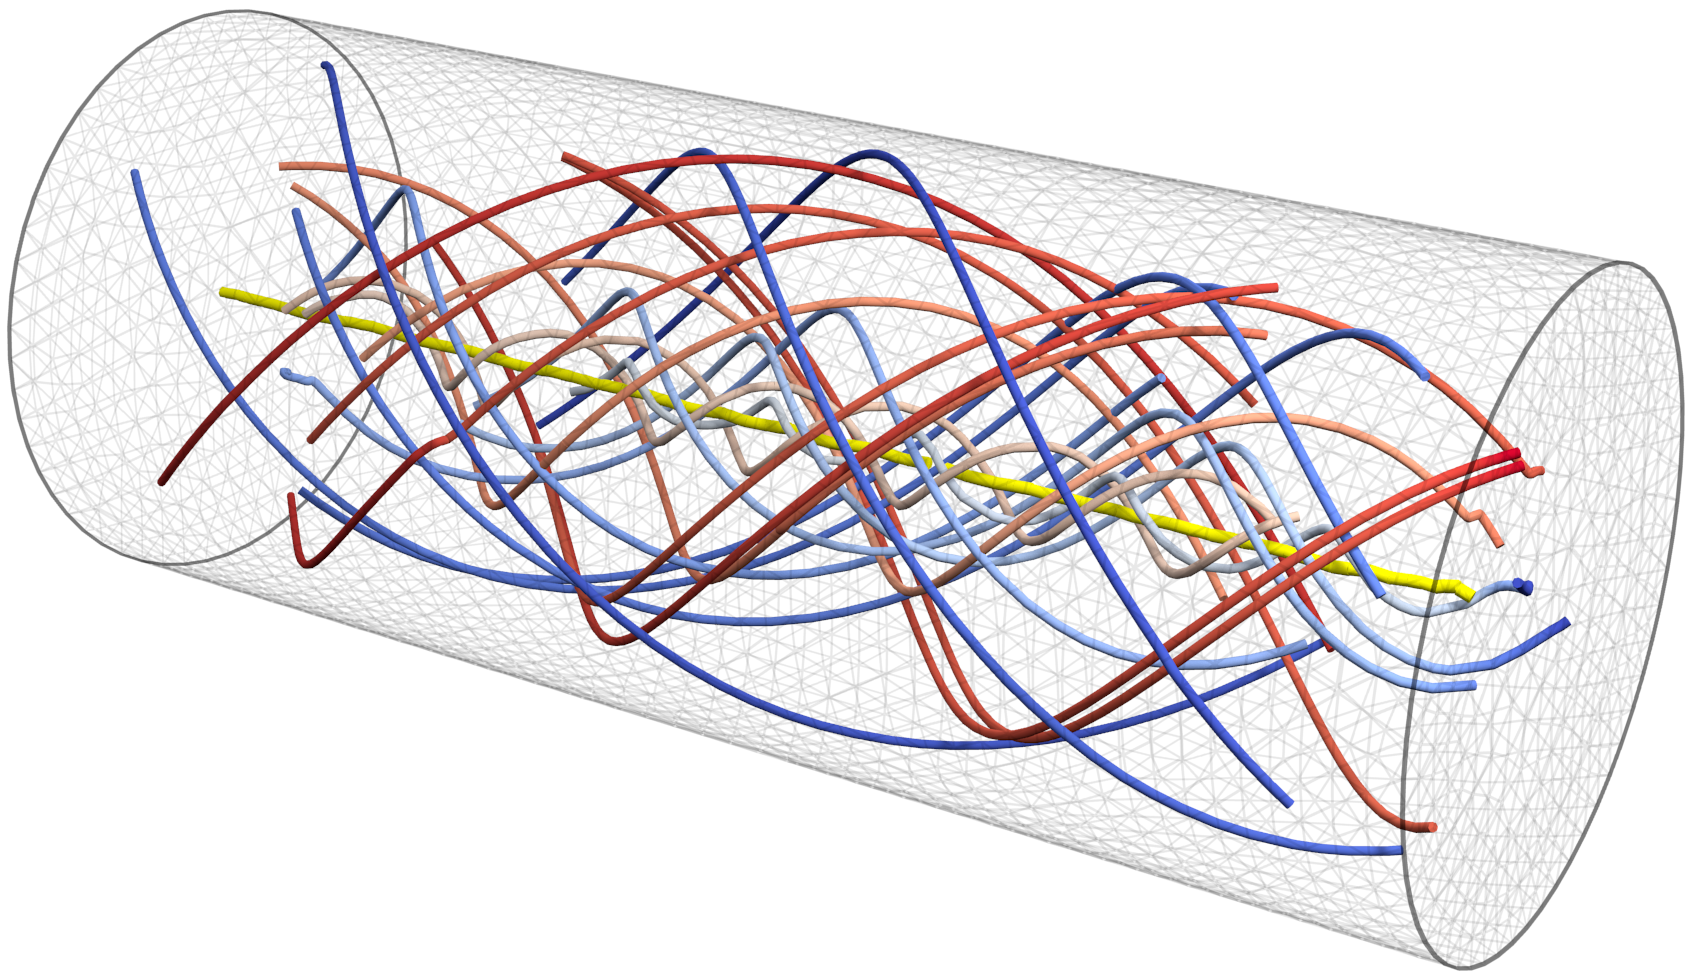
\includegraphics[width=\figurewidth]{figures/torque_tube_lines.png}
    };
    \begin{scope}[
        shift=(img.south west), % origin is lower left corner
        x={($(img.south east)-(img.south west)$)}, % x axis is lower side
        y={($(img.north west)-(img.south west)$)}] % y axis is left side
        % uncomment the following three lines to show a helper grid that helps
        % with finding coordinates
        % \draw[help lines, opacity=0.5, xstep=.01,ystep=.01] (0,0) grid (1,1);
        % \draw[thin, xstep=.1,ystep=.1] (0,0) grid (1,1);
        % \foreach \x in {0,...,9} { \node [anchor=north] at (\x/10,0) {0.\x}; }
        % \foreach \y in {0,...,9} { \node [anchor=east] at (0,\y/10) {0.\y}; }
        % draw stuff on image
        % (0, 0) is lower left corner, (1, 1) is upper right
        \node at (0.916,0.37) {
            \begin{tikzpicture}
                \draw[-latex, ultra thick, black, rotate=76] (0,0)
                arc[x radius = 2.6cm, y radius = 0.8cm, start angle= 60, end angle= -255];
            \end{tikzpicture}
        };

        \node at (0.123,0.705) {
            \begin{tikzpicture}
                \draw[-latex, ultra thick, black, rotate=76] (0,0)
                arc[x radius = 2.02cm, y radius = 1.385cm, start angle= -255, end angle= 60];
            \end{tikzpicture}
        };
    \end{scope}
\end{tikzpicture}
    % \vspace*{-9mm}
    \caption{Tensor field lines in a stress tensor field induced by
             applying a torque to a cylindrical shaft. Field lines of both major
             (blue) and minor (red) eigenvectors show a swirling behavior around
             a common core line (yellow).}
    \label{fig:tube_lines}
\end{figure}
%
In particular, we make the following contributions:
%
\begin{itemize}
    \item  We give a rigorous definition of tensor core lines and show that
    indeed the definition gives structurally stable line structures.
    %
    \item We provide a numerical algorithm for the extraction of tensor core
    lines from piecewise linear tensor fields.
    %
    \item We introduce a filter criterion based on numerical stability to
    separate significant and insignificant tensor core lines.
    %
    \item We show tensor core lines in mechanical stress tensor fields,
    interpret them and compare them with degenerate lines where two eigenvalues
    are equal.
\end{itemize}
%
We introduce tensor core lines in \cref{sec:tcl_theory} and study their
properties.
%
We then present our algorithm for extracting tensor core lines in
\cref{sec:extracting_tensor_lines}.
%
We show our results on several stress tensor fields in \cref{sec:tcl_results}
and study the performance, robustness and relation to degenerate lines.
%
As it turns out, our algorithm is sufficiently generic to be applied to the
extraction of \ac{PEV} lines and degenerate lines as well.
%
We show how this can be done in \cref{sec:computing_pev_and_degenerate_lines}
and close with a discussion in \cref{sec:tcl_discussion}.
%
% section introduction (end)